\bookchapter{Networking from the Command Line}\label{ch:linux7}

\section*{Explanation}
Almost everything on a robot talks over a network: your SSH session, the camera stream to your laptop, ROS~2 messages between computers, the WiFi connection of the team. When something does not connect, you need a method to find out \emph{where} it breaks. This chapter gives you the vocabulary and a small set of tools.

\subsection*{Addresses, subnets and ports}
Every network interface has an \textbf{IP address}, for example \texttt{192.168.10.5}: four numbers from $0$ to $255$ (four bytes). The address is split into a \textbf{network part} and a \textbf{host part}. The \textbf{prefix length} written after a slash says how many of the $32$ bits belong to the network: \texttt{192.168.10.5/24} means that the first $24$ bits (the first three numbers) name the network, and the last $8$ bits name the computer. The same information is the \textbf{netmask} (\texttt{255.255.255.0} for \texttt{/24}).

\begin{center}
\renewcommand{\arraystretch}{1.2}
\begin{tabular}{lccc}
\textbf{prefix} & \textbf{netmask} & \textbf{addresses} & \textbf{usable hosts}\\ \hline
\texttt{/24} & 255.255.255.0 & 256 & 254\\
\texttt{/16} & 255.255.0.0 & 65\,536 & 65\,534\\
\texttt{/26} & 255.255.255.192 & 64 & 62\\
\texttt{/30} & 255.255.255.252 & 4 & 2\\
\end{tabular}
\end{center}
Two addresses in each network are reserved: the first (the network address, host bits all $0$) and the last (the \textbf{broadcast} address, host bits all $1$), hence ``$-2$''.

\begin{example}
\texttt{192.168.10.5/24}: the network is \texttt{192.168.10.0}, the broadcast address \texttt{192.168.10.255}, the usable hosts are \texttt{192.168.10.1} to \texttt{.254}. The address \texttt{192.168.10.70/26} lies in the block of $64$ addresses from \texttt{.64} to \texttt{.127}: network \texttt{192.168.10.64}, broadcast \texttt{192.168.10.127}.
\end{example}

Computers in the \emph{same} network talk directly. For everything else they send the packets to the \textbf{gateway} (the \textbf{router}), which forwards them (Figure~\ref{fig:l7_net}). Addresses starting with \texttt{192.168.}, \texttt{10.} or \texttt{172.16--31.} are \textbf{private}: they are used inside local networks and not routed on the internet.

\begin{center}
\begin{tikzpicture}[box/.style={draw,rounded corners,thick,minimum height=1.0cm,minimum width=2.4cm,align=center,font=\small},>={Stealth[length=2.5mm]}]
  \node[box,fill=blue!10] (L) at (0,1.0) {laptop\\{\scriptsize \texttt{192.168.10.20}}};
  \node[box,fill=green!12] (R) at (0,-1.0) {robot\\{\scriptsize \texttt{192.168.10.5}}};
  \node[box,fill=orange!18] (G) at (5.0,0) {router\\{\scriptsize \texttt{192.168.10.1}}};
  \node[box,fill=gray!12] (I) at (10.0,0) {internet\\{\scriptsize \texttt{8.8.8.8}, \dots}};
  \draw[thick] (L) -- (G); \draw[thick] (R) -- (G); \draw[->,thick] (G) -- (I);
  \draw[thick,rounded corners,gray] (-1.7,-2.0) rectangle (6.5,2.0);
  \node[font=\scriptsize,gray,anchor=north west] at (-1.65,2.0) {network \texttt{192.168.10.0/24}};
\end{tikzpicture}
\captionof{figure}{Laptop and robot are in the same \texttt{/24} network and talk directly. Packets for the internet go to the router (the default gateway).}\label{fig:l7_net}
\end{center}

A \textbf{port} is a number from $0$ to $65535$ that selects a service on a computer, like an apartment number in a building: the address finds the computer, the port finds the program. \textbf{TCP} provides a reliable connection (SSH, web); \textbf{UDP} sends single messages without a connection (video, ROS~2 discovery). Well-known ports: \texttt{22} SSH, \texttt{53} DNS, \texttt{80} HTTP, \texttt{123} time, \texttt{443} HTTPS. ROS~2 (Part~V) uses UDP ports starting at \texttt{7400}.

\textbf{Names.} People use names such as \texttt{k1} or \texttt{github.com}. \textbf{DNS} translates names into addresses. On small networks \textbf{mDNS} lets machines announce themselves as \texttt{name.local} (e.g.\ \texttt{ssh robot@k1-brain.local}). The file \texttt{/etc/hosts} holds your own fixed name-to-address entries.

\section*{Looking at your own network}
\begin{verbatim}
$ ip -br addr                   # short overview of all interfaces
lo      UNKNOWN  127.0.0.1/8
eth0    UP       192.168.10.5/24
wlan0   DOWN
$ ip route                      # the routing table
default via 192.168.10.1 dev eth0
192.168.10.0/24 dev eth0 proto kernel scope link src 192.168.10.5
$ ip neigh                      # neighbours seen in the local network
$ resolvectl status             # DNS servers in use
$ hostname -I                   # just my addresses
\end{verbatim}
\texttt{lo} is the \textbf{loopback} interface: \texttt{127.0.0.1} (\texttt{localhost}) always means ``this computer''. The line \texttt{default via 192.168.10.1} says that everything that is not in the local network goes to the router at \texttt{192.168.10.1}.

\textbf{WiFi} is managed by \textbf{NetworkManager}: \verb|nmcli device wifi list|, \verb|nmcli device wifi connect SSID password PASS|, \verb|nmcli connection show|. On servers the configuration is often in YAML files under \texttt{/etc/netplan/} (apply with \verb|sudo netplan apply|); a fixed address looks like \texttt{addresses: [192.168.10.5/24]}.

\section*{Testing connections}
\begin{verbatim}
$ ping -c 4 192.168.10.1           # 4 echo requests to the router
64 bytes from 192.168.10.1: icmp_seq=1 ttl=64 time=0.9 ms
...
4 packets transmitted, 4 received, 0% packet loss
rtt min/avg/max/mdev = 0.8/1.0/1.3/0.2 ms
$ traceroute 8.8.8.8               # which routers on the way (or: mtr)
$ nc -zv 192.168.10.5 22           # is port 22 reachable?
$ curl -I https://example.org      # fetch only the HTTP header
$ curl -O https://host/file.tar.gz # download a file
\end{verbatim}
\texttt{ping} sends small test packets and measures the \textbf{round-trip time} (latency) in milliseconds. Look at the \textbf{packet loss}: on a wired network it should be $0\,\%$. A WiFi link with $5\,\%$ loss or jumping latencies explains laggy teleoperation. (Some firewalls drop ping, so a missing answer is not always an error.)

\textbf{What is listening on this machine?}
\begin{verbatim}
$ sudo ss -tulpn                   # TCP/UDP, listening, program, numeric
Netid State  Local Address:Port  Process
tcp   LISTEN 0.0.0.0:22          users:(("sshd",pid=812))
tcp   LISTEN 127.0.0.1:8080      users:(("python",pid=1423))
udp   UNCONN 0.0.0.0:7400        users:(("ros2",pid=2210))
\end{verbatim}
\texttt{0.0.0.0:22} means that SSH accepts connections on \emph{all} interfaces. \texttt{127.0.0.1:8080} listens only on the loopback interface, so it is reachable only from this machine (or through an SSH tunnel, Chapter~\ref{ch:linux3}). Use \texttt{ss -tn} to see the established connections.

\section*{Finding the problem: the ladder}
When a connection does not work, go up the ladder step by step and stop at the first step that fails (Figure~\ref{fig:l7_ladder}):

\begin{center}
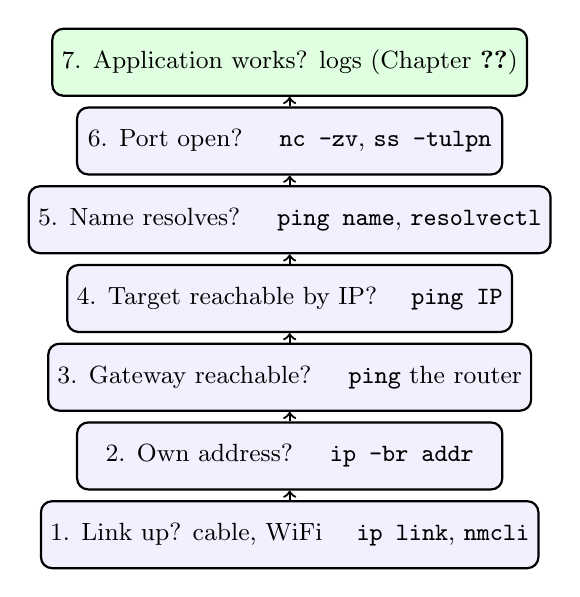
\begin{tikzpicture}[st/.style={draw,rounded corners,thick,minimum width=5.4cm,minimum height=0.85cm,font=\small,align=left,fill=blue!6}]
  \node[st] (a) at (0,0) {1. Link up? cable, WiFi \quad \texttt{ip link}, \texttt{nmcli}};
  \node[st] (b) at (0,1.0) {2. Own address? \quad \texttt{ip -br addr}};
  \node[st] (c) at (0,2.0) {3. Gateway reachable? \quad \texttt{ping} the router};
  \node[st] (d) at (0,3.0) {4. Target reachable by IP? \quad \texttt{ping IP}};
  \node[st] (e) at (0,4.0) {5. Name resolves? \quad \texttt{ping name}, \texttt{resolvectl}};
  \node[st] (f) at (0,5.0) {6. Port open? \quad \texttt{nc -zv}, \texttt{ss -tulpn}};
  \node[st,fill=green!12] (g) at (0,6.0) {7. Application works? logs (Chapter~\ref{ch:linux5})};
  \foreach \a/\b in {a/b,b/c,c/d,d/e,e/f,f/g}{\draw[->,thick] (\a) -- (\b);}
\end{tikzpicture}
\captionof{figure}{Go up the ladder. The first failing step tells you what to look at.}\label{fig:l7_ladder}
\end{center}
\begin{center}
\renewcommand{\arraystretch}{1.25}
\begin{tabular}{p{5.0cm}p{8.6cm}}
\textbf{Symptom} & \textbf{Probable cause}\\ \hline
\texttt{ping IP} works, \texttt{ping name} fails & DNS problem. Check \texttt{resolvectl status}, try another DNS server.\\
\texttt{ping} works, SSH \emph{refused} & \texttt{sshd} not running or wrong port (\texttt{ss -tulpn} on the target).\\
\texttt{ping} works, SSH \emph{times out} & A firewall drops the packets (e.g.\ \texttt{ufw}).\\
Only some computers reachable & Different subnets or no route; look at \texttt{ip route}.\\
Works, but laggy & Packet loss or high latency: \texttt{ping}, WiFi signal, \texttt{iperf3}.\\
\end{tabular}
\end{center}

\subsection*{Firewall, bandwidth, and ROS~2}
\begin{itemize}[nosep]
  \item \textbf{ufw} is the simple Ubuntu firewall: \verb|sudo ufw status|, \verb|sudo ufw allow 22/tcp|, \verb|sudo ufw enable|. Careful: enable the SSH rule \emph{before} enabling the firewall on a remote machine, or you lock yourself out.
  \item \textbf{Bandwidth:} \texttt{iperf3 -s} on one machine and \texttt{iperf3 -c HOST} on the other measure the throughput. A camera stream with $640\times480$ pixels and $3$ bytes each at $30$ frames per second needs $640\cdot480\cdot3\cdot30\approx27.6$\,MB/s ($221$\,Mbit/s) if it is \emph{not compressed}. This is why video is compressed (JPEG, H.264).
  \item \textbf{Watching traffic:} \verb|sudo tcpdump -i eth0 port 22| shows packets, a last resort when nothing else explains the problem.
  \item \textbf{ROS~2} finds other computers by multicast on the local network. All computers must be in the same subnet, use the same \texttt{ROS\_DOMAIN\_ID}, and WiFi that blocks multicast is a classic reason why nodes do not see each other.
  \item \textbf{Time:} all computers should agree on the time (needed for logs, certificates and sensor fusion). Ubuntu keeps the clock with a time service (\texttt{chrony} on new installations); check with \verb|timedatectl|.
\end{itemize}

\begin{aibox}
``The robot is not reachable'' has only a handful of causes, and the ladder finds them in two minutes. Before a competition write down the address plan (IP range, router, who has which fixed address) and check that every robot answers to \texttt{ping}, \texttt{ssh} and your video port.
\end{aibox}

\section*{Practice problems}
\begin{enumerate}[label=\textbf{\thechapter.\arabic*}]
  \item For \texttt{192.168.10.5/24}: give the netmask, the network address, the broadcast address and the number of usable host addresses.
  \item Are \texttt{192.168.10.5} and \texttt{192.168.11.7} in the same network if the prefix is (a) \texttt{/24}, (b) \texttt{/16}?
  \item The address \texttt{192.168.10.70/26}: which block of addresses does it belong to? Give the network and broadcast address.
  \item How many usable hosts does a \texttt{/30} network have, and what is it often used for?
  \item Which commands show (a) your IP addresses, (b) the default gateway, (c) the program that listens on port $8080$?
  \item \texttt{ping 8.8.8.8} works but \texttt{ping github.com} gives \texttt{Name or service not known}. Which step of the ladder fails, and what do you check?
  \item \texttt{ssh robot@192.168.10.5} says \texttt{Connection refused}, while \texttt{ping} works. What does this mean, and how do you find out more (on the robot)?
  \item A service prints \verb|127.0.0.1:8080| in \texttt{ss -tulpn}. Can your laptop connect to \texttt{http://192.168.10.5:8080}? How can you reach it anyway?
  \item An uncompressed camera stream has $1280\times720$ pixels, $3$ bytes per pixel, $15$ frames per second. How many Mbit/s is that? Does it fit through a $100$\,Mbit/s link?
  \item[\textbf{\thechapter.10}$\star$] You enable \texttt{ufw} on the robot over SSH and your session freezes. What did you probably forget, and how do you avoid it?
\end{enumerate}
